 \documentclass[10pt, table, dvipsnames,xcdraw, handout]{beamer}
\usetheme[progressbar=frametitle]{metropolis}
\usepackage{appendixnumberbeamer}
\usetikzlibrary{arrows.meta, positioning, quotes}
\usepackage[shortlabels]{enumitem}
\usepackage{xcolor}
\usepackage{mathtools}


\usepackage{cancel}

\newcommand\hcancel[2][black]{\setbox0=\hbox{$#2$}%
\rlap{\raisebox{.45\ht0}{\textcolor{#1}{\rule{\wd0}{1pt}}}}#2} 


\usepackage{booktabs}
\usepackage[scale=2]{ccicons}

\usepackage{pgfplots}
\usepgfplotslibrary{dateplot}

\usepackage{xspace}
\newcommand{\themename}{\textbf{\textsc{metropolis}}\xspace}
\newcommand{\cb}{\cellcolor{blue!25}}


% Notation:
\newcommand{\cT}{\ensuremath{\mathcal{T}}}
\newcommand{\cD}{\ensuremath{\mathcal{D}}}
\newcommand{\cX}{\ensuremath{\mathcal{X}}}
\newcommand{\cY}{\ensuremath{\mathcal{Y}}}
\newcommand{\cZ}{\ensuremath{\mathcal{Z}}}
\newcommand{\cH}{\ensuremath{\mathcal{H}}}
\newcommand{\cG}{\ensuremath{\mathcal{G}}}

\newcommand{\bR}{\ensuremath{\mathbb{R}}}
\newcommand{\bN}{\ensuremath{\mathbb{N}}}
\newcommand{\bP}{\ensuremath{\mathbb{P}}}
\newcommand{\bT}{\ensuremath{\mathbb{T}}}
\newcommand{\bL}{\ensuremath{\mathbb{L}}}

\newcommand{\bfX}{\ensuremath{\mathbf{X}}}
\newcommand{\bfY}{\ensuremath{\mathbf{Y}}}
\newcommand{\bfy}{\ensuremath{\mathbf{y}}}

% Tikz seys
\tikzset{cross/.style={cross out, draw, 
         minimum size=2*(#1-\pgflinewidth), 
         inner sep=0pt, outer sep=0pt}}

\title{Machine Learning I}
\subtitle{Lecture 6: Iterative Methods}
% \date{\today}
\date{}
\author{Nathaniel Bade}
\institute{Northeastern University Department of Mathematics}
% \titlegraphic{\hfill\includegraphics[height=1.5cm]{logo.pdf}}

\begin{document}

\maketitle

\begin{frame}{Table of contents}
  \setbeamertemplate{section in toc}[sections numbered]
  \tableofcontents[hideallsubsections]
\end{frame}


%%%%%%%%%%%%%% Slidshow Start %%%%%%%%%%%%%% 

\section{The need for iterative methods}
\begin{frame}[fragile]{More complicated models}
  \begin{minipage}[t][0.5\textheight][t]{\textwidth}
	\centering \includegraphics[height=0.5\textheight]{L10Polynomial.png} 
  \end{minipage}
  \vfill
\begin{minipage}[t][0.5\textheight][t]{\textwidth}
Not everything in the world is linear. We saw last lecture that polynomial functions can be fit by performing linear regression on synthetic features $X_{i_1}^{d_1}\ldots X_{i_r}^{d_r}$. \pause The obvious problem is that degree $d$ polynomials on $p$ features lead to 
$$
\textbf{Number of Features:}\hspace{2em}\binom{d+p}{d}\,.
$$
\end{minipage}
\end{frame}





\begin{frame}[fragile]{More complicated models}
  \begin{minipage}[t][0.5\textheight][t]{\textwidth}
	\centering \includegraphics[height=0.5\textheight]{L10Polynomial.png} 
  \end{minipage}
  \vfill
\begin{minipage}[t][0.5\textheight][t]{\textwidth}
As an example, on the MNIST data set there are 308,505 degree 2 polynomials and 80,931,145 degree three polynomials. \pause Without a principled reason, inverting a matrix to solve such problems quickly becomes prohibitive. 
\end{minipage}
\end{frame}








\begin{frame}[fragile]{More complicated models}
  \begin{minipage}[t][0.5\textheight][t]{\textwidth}
	\centering \includegraphics[height=0.5\textheight]{L10Polynomial.png} 
  \end{minipage}
  \vfill
\begin{minipage}[t][0.5\textheight][t]{\textwidth}
How can we fit such models when the functions are too complicated to yield a close form solution for the minimia? \pause When the number of variables is too large to efficiently use linear methods? \pause When the models themselves may not have closed form formula?\pause
\end{minipage}
\end{frame}


\begin{frame}[fragile]{More complicated models}
  \begin{minipage}[t][0.5\textheight][t]{\textwidth}
	\centering \includegraphics[height=0.5\textheight]{L10Polynomial.png} 
  \end{minipage}
  \vfill
\begin{minipage}[t][0.5\textheight][t]{\textwidth}
In this lecture we're going to being talking about how to fit more complicated functions. We will start by canvasing several methods for our linear classifiers, and then show how to extend these results to polynomials and exponential functions. 
\end{minipage}
\end{frame}





\section{Gradient Decent}

\begin{frame}[fragile]{Gradient Decent}
  \begin{minipage}[t][0.5\textheight][t]{\textwidth}
	\centering \includegraphics[height=0.5\textheight]{L10Gradiant.png} 
  \end{minipage}
  \vfill
\begin{minipage}[t][0.5\textheight][t]{\textwidth}
Gradient decent is an incredibly general method of finding the minima of functions. Lets recall some facts from calculus: Let $F(x)$ be a differentiable function depending on a vector of parameters $x$, so $F:\bR^k\to \bR$. Then, the gradient $\nabla F$ always points in the direction of greatest increase.
\end{minipage}
\end{frame}






\begin{frame}[fragile]{Gradient Decent}
  \begin{minipage}[t][0.5\textheight][t]{\textwidth}
	\centering \includegraphics[height=0.5\textheight]{L10GradiantDecent1.png} 
  \end{minipage}
  \vfill
\begin{minipage}[t][0.5\textheight][t]{\textwidth}
This means that if we want to find a minimum, we can follow $-\nabla F$ downhill. Concretely, for $\eta$ sufficiently small, 
$$
F(x - \eta \nabla F) \approx F(x) - \eta\, \nabla F \cdot  \nabla F  = F(x) - \eta\, ||\nabla F ||^2 < F(x) \,.
$$
If $F$ is always positive and not at a minimum, than a sufficiently small step in the $\nabla F$ direction will always decrease $F$. 
\end{minipage}
\end{frame}





\begin{frame}[fragile]{Gradient Decent}
  \begin{minipage}[t][0.5\textheight][t]{\textwidth}
	\centering \includegraphics[height=0.5\textheight]{L10GradiantDecent1.png} 
  \end{minipage}
  \vfill
\begin{minipage}[t][0.5\textheight][t]{\textwidth}
Algorithmically, at each $x^{(n)}$ we compute the next step by
$$
x^{(n+1)} = x^{(n)} - \eta \nabla F\,,
$$
where $\eta > 0$ is the \textbf{learning rate} hyperparameter.  
\end{minipage}
\end{frame}




\begin{frame}[fragile]{Gradient Decent}
  \begin{minipage}[t][0.5\textheight][t]{\textwidth}
	\centering \includegraphics[height=0.5\textheight]{L10GradiantDecent2.png} 
  \end{minipage}
  \vfill
\begin{minipage}[t][0.5\textheight][t]{\textwidth}
The learning rate $\eta$ determines proportionally how far of a step we take in the $-\nabla F$ direction. If $\eta$ is too small we may find that the algorithm appears to converge but does so to a point that isn't an actual minimum.
\end{minipage}
\end{frame}




\begin{frame}[fragile]{Gradient Decent}
  \begin{minipage}[t][0.5\textheight][t]{\textwidth}
	\centering \includegraphics[height=0.5\textheight]{L10GradiantDecent3.png} 
  \end{minipage}
  \vfill
\begin{minipage}[t][0.5\textheight][t]{\textwidth}
On the other hand, if $\eta$ is too large we may actually walk away from the minimum. \pause We will see an example for linear regression explicitly. 
\end{minipage}
\end{frame}




\begin{frame}[fragile]{Gradient Decent}
  \begin{minipage}[t][0.5\textheight][t]{\textwidth}
	\centering \includegraphics[height=0.5\textheight]{L10GradiantDecent4.png} 
  \end{minipage}
  \vfill
\begin{minipage}[t][0.5\textheight][t]{\textwidth}
Of course, gradient decent is a greedy method and so if $\eta$ is too small it may miss a global minimum in favor of a local one. \pause If we want to guarantee that gradient decent can actually find the minimum, we will need some extra assumptions on our hypothesis class and loss function. RSS for Linear Regression turns out to only have a single minimum. 
\end{minipage}
\end{frame}





\begin{frame}[fragile]{Batch Gradient Decent}
If we compute the gradient using all of the training data it is called \textbf{batch gradient decent}. For mean squared error, 
$$
MSE(\beta) = \frac{1}{N}(\bfy  - \bfX\beta)^T (\bfy  - \bfX\beta)
$$ 
a formula is readily available. \pause Choosing to represent $\nabla_\beta MSE(\beta)$ as a $p+1$ column vector, the gradient is
$$
\nabla_\beta MSE = -\frac{2}{N}\bfX^T (\bfy  - \bfX\beta)\,.
$$ \pause
The update step for the parameters $\beta$ is
$$
\beta^{(n+1)} = \beta^{(n)} +\eta \frac{2}{N}\bfX^T (\bfy  - \bfX\beta^{(n)})\,.
$$

\end{frame}




\begin{frame}[fragile]{Batch Gradient Decent}
  \begin{minipage}[t][0.5\textheight][t]{\textwidth}
	\centering \includegraphics[width=\textwidth]{L10GradiantDecent5.png} 
  \end{minipage}
  \vfill
\begin{minipage}[t][0.5\textheight][t]{\textwidth}
We see the results for MSE and linear regression above. If $\eta$ is too low, convergence is slow (possibly to the point of being undetectable). \pause If it is too large, the fit is actually repelled by the minimum. 
\end{minipage}
\end{frame}





\begin{frame}[fragile]{Batch Gradient Decent}
  \begin{minipage}[t][0.5\textheight][t]{\textwidth}
	\centering \includegraphics[width=\textwidth]{L10GradiantDecent5.png} 
  \end{minipage}
  \vfill
\begin{minipage}[t][0.5\textheight][t]{\textwidth}
In addition to $\eta$, we must decide how many iterations we will use. Optimally, we would like to find a learning rate that causes convergence in a small number of iterations. 

\pause The learning rate can be fixed (say by performing a grid search to find the best $\eta$) or variable, starting large and then lowering to attempt to avoid both falling into and being repelled by local minimia. 
\end{minipage}
\end{frame}




\begin{frame}[fragile]{Batch Gradient Decent}
  \begin{minipage}[t][0.5\textheight][t]{\textwidth}
	\centering \includegraphics[width=\textwidth]{L10GradiantDecent5.png} 
  \end{minipage}
  \vfill
\begin{minipage}[t][0.5\textheight][t]{\textwidth}
Similarly, the number of iterations can be fixed, or we can choose to stop when, say, $||\nabla \beta|| <\epsilon$ for some \textbf{tolerance} $\epsilon$. \pause

It can be show that for $MSE$ with fixed $\eta$, the convergence rate is approximately $O\left(\frac{1}{\text{itter}}\right)\,.$\pause That is, to decrease the tolerance $\epsilon$ by $\frac12$ we must double the number of iterations. 
\end{minipage}
\end{frame}



\begin{frame}[fragile]{Checklist for implementing gradient decent}
Checklist for implementing gradient decent:

Let $f(X, \beta)$ be a positive function that depends on data $\mathbf{X}$ and parameters $\beta$. Let $F(\mathbf{X},\beta) = \sum_{i=1}^N f(x_i, \beta)$. Then GD on $F$ is

\textbf{Step 1:} Find an expression for $\nabla_\beta F$. 

\textbf{Step 2:} Set an initial guess for $\beta^{(0)}$ and fix a learning rate $\eta$. 

\textbf{Step 3:} For each $n$, compute $\beta^{(n+1)} = \beta^{(n)} - \eta \nabla_\beta F$

\textbf{Step 4:} Stop when $\eta ||\nabla_\beta F||$ is sufficiently small, after a fixed number of steps, of when $F$ is sufficiently small. Alternatively, define a \textbf{learning schedule} for $\eta$ which gradually lowered $\eta$ as $n$ gets large. 
\end{frame}




\section{Stochastic Gradient Decent}

\begin{frame}[fragile]{Batch Gradient Decent}
The main problem with batch gradient decent is that all the training data is used to compute the parameters on each iteration. This slows down training considerably when the dataset is large. \pause

At the opposite end, \textbf{Stochastic Gradient Decent} (SGD) picks a random element of the training set and uses that to update, like the perception algorithm. SGD a much faster than batch GD since it only needs a single element to train on. The tradeoff is it is much more random.\pause

If $f(X, \beta)$ is a positive function that depends on data $\mathbf{X}$ and parameters $\beta$. Let $F(\mathbf{X},\beta) = \sum_{i=1}^N f(x_i, \beta)$. Then SGD updates $\beta^{(n)}$ by randomly sampling $x\sim \mathbf{X}$ and computing
$$
\beta^{(n+1)} = \beta^{(n)} - \eta\nabla f(x)\,. 
$$
Of course, $\beta$ will take many more steps to converge, but the computation at each step will be much simpler. 
\end{frame}



\begin{frame}[fragile]{Batch Gradient Decent}
  \begin{minipage}[t][0.5\textheight][t]{\textwidth}
	\centering \includegraphics[height=.5\textheight]{L10StocGradDecent.png} 
  \end{minipage}
  \vfill
\begin{minipage}[t][0.5\textheight][t]{\textwidth}
Comparing gradient decent and stochastic gradient decent, gradient decent will be much more stable, usually plodding along directly towards to nearest local minimum and getting stuck there. SGD on the other hand is much more random, and may walk towards or away at each step.
\end{minipage}
\end{frame}





\begin{frame}[fragile]{Stochastic Gradient Decent}
  \begin{minipage}[t][0.5\textheight][t]{\textwidth}
	\centering \includegraphics[width=.8\textwidth]{L10SGD.png} 
  \end{minipage}
  \vfill
\begin{minipage}[t][0.5\textheight][t]{\textwidth}
SGD is much more likely to avoid getting stuck in local minimia, but on the other hand it doesn't tend to settle down (even in a global minimum). As a result it is almost necessary to gradually lower the learning rate $\eta$ as we train. The function that determines $\eta$ is called the \textbf{learning schedule}. 
\end{minipage}
\end{frame}






\begin{frame}[fragile]{Stochastic Gradient Decent}
  \begin{minipage}[t][0.5\textheight][t]{\textwidth}
	\centering \includegraphics[width=\textwidth]{L10SGD1.png} 
  \end{minipage}
  \vfill
\begin{minipage}[t][0.5\textheight][t]{\textwidth}
Training on the entire data set all at once (GD) or one at a time (SGD) called a \textbf{training epoch}. It is customary to train multiple epochs, resetting the learning schedule each time.  

Although this produces many training steps, each step is computationally simple. 
\end{minipage}

\end{frame}







\begin{frame}[fragile]{Stochastic Gradient Decent}
  \begin{minipage}[t][0.5\textheight][t]{\textwidth}
	\centering \includegraphics[width=\textwidth]{L10SGD2.png} 
  \end{minipage}
  \vfill
\begin{minipage}[t][0.5\textheight][t]{\textwidth}
Finally \textbf{minibatch gradient decent} splits the difference between SGD and GD, training in epochs of $m$ subsets of size $n$, where $m\times n = N$. All three methods are implemented in sci-kit learn and (for convex problems) yield the same results. \pause

The batch size $m$ provides a nonlinear trade off between the number of iterations to convergence and the number complexity of each iterative step. 
\end{minipage}
\end{frame}



\begin{frame}[fragile]{Stochastic Gradient Decent}
  \begin{minipage}[t][0.5\textheight][t]{\textwidth}
	\centering \includegraphics[width=\textwidth]{L10SGD2.png} 
  \end{minipage}
  \vfill
\begin{minipage}[t][0.5\textheight][t]{\textwidth}
In the above, the lines are colored by epochs. Notice that after 5 epochs we are closer to the true center line, but it will take about 10 more epochs to get within 1\% of the RSS fit.  
\end{minipage}
\end{frame}



\begin{frame}[fragile]{Checklist for implementing batch gradient decent}
Checklist for implementing batch gradient decent or SGD:

Let $f(X, \beta)$ be a positive function that depends on data $\mathbf{X}$ and parameters $\beta$. Let $m<N$ be the batch size and let $F_M(\mathbf{X},\beta) = \sum_{i=1}^M f(x_i, \beta)$. Then GD on $F$ is

\textbf{Step 1:} Find an expression for $\nabla_\beta F_M$. 

\textbf{Step 2:} Set an initial guess for $\beta^{(0)}$ and fix a learning rate $\eta$. 

\textbf{Step 3:} Shuffle $\mathbf{X}$ and split it into $k$ batched of $M$ unique data points denoted $\mathbf{X}_j$. For each $n$, compute $\beta^{(k n+j)}$ by $\beta^{(n+1)} = \beta^{(n)} - \eta \nabla_\beta F_M(\mathbf{X}_j)$.

\textbf{Step 4:} Stop when $\eta ||\nabla_\beta F||$ is sufficiently small, after a fixed number of steps, of when $F$ is sufficiently small. Alternatively, define a \textbf{learning schedule} for $\eta$ which gradually lowered $\eta$ as $n$ gets large. 
\end{frame}



\section{Newtons Method}


\begin{frame}[fragile]{Newtons Method}
Newtons Method is an iterative method of finding zeros of differential functions. By applying it to the first derivative of a function we can use it to find minima, maxima and saddle points. \pause

Newtons method is considerably faster than gradient decent but relies on finding second derivatives of the loss function. This means that not only must the loss function be twice differentiable, but a formula should be available for all second derivatives. \pause

As a result, Newtons method isn't as widely used as GD, SGD and other solvers, but when it can be implemented it tends to be superior. 
\end{frame}


\begin{frame}[fragile]{Newtons Method}
In one variable, we try to find a zero of $f(x)$ by successive approximations of $f(x)$ by it's Taylor polynomial. 

\pause Starting with $x$, we try to find an improved guess $x+\eta$ by Taylor expanding $f(x+\eta)$ around $x$:
$$
f(x+\eta) \approx f(x)+\eta f'(x) = 0\,.
$$\pause
Solving for $\delta =- f(x)/f'(x)$, we have an ``improved'' guess $x_{new} = x- f(x)/f'(x)$ for the location of the zero. \pause We then iterate until we have arrived at a zero. It can be proved that under reasonable assumptions on $f(x)$ we always will converge to a zero. 
\end{frame}



\begin{frame}[fragile]{Multivariate Newtons Method}
For higher dimensional functions, we proceed exactly as before: Let $f(x)$ be differentiable. Expanding $f( x +  \eta)$ around $ x$, we find
$$
f( x+\eta) \approx  f(x) + J(x) \eta = 0\,,
$$
where $J_{ij} = \frac{\partial f_i}{\partial x_j}$ is the Jacobean matrix (gradient if $f(x)\in \mathbb{R}$). \pause If $J(x)$ is invertible, we can solve for
$$
x_{new} =  x - J^{-1}( x) f(x) \,.
$$
Note, unless $f:\bR^d\to\bR^d$ $J(x)$ will almost certainly not be even partially invertible.
\end{frame}


\begin{frame}[fragile]{Optimization via Newtons Method}
For a single valued multivariate function $f(x)$, we can use Newtons method to perform optimization. Since optimization is just finding $\nabla f(x) = 0$, we write
$$
\nabla f(x+\eta) \approx \nabla f(x)  + H_f(x) \eta =0\,
$$
where $H_f(x) = (\frac{\partial f}{\partial x_i\partial x_j})_{ij}$ is the Hessian matrix. \pause At each iteration then we update $x_{old}$ to
$$
x_{new} = x_{old} - H^{-1}_f(x)\nabla f(x)\,.
$$\pause
Note, Newtons Method converges much faster than gradient decent, but requires computing higher derivatives which might not exist, or may be hard to compute. As a result, it often cannot be used. 
\end{frame}



\begin{frame}[fragile]{Example: Linear Regression Via Newtons Method}
Lets solve linear regression using Newtons Method. The gradient of $MSE = \frac1N(\bfy-\bfX\beta)^T (\bfy-\bfX\beta)$ is
$$
\nabla MSE =  -\frac2N\bfX^T(\bfy - \bfX\beta)\,,
$$\pause
and the Hessian is the $(p+1)\times (p+1)$ matrix
$$
H_{MSE} = \frac{2}{N} \bfX^T\bfX\,.
$$\pause
Given an initial $\beta^{(0)}$, the update rule is
$$
\beta^{(n+1)} = \beta^{(n)} + (\frac{2}{N} \bfX^T\bfX)^{-1}\frac2N\bfX^T(\bfy - \bfX\beta^{(n)}) \pause = \beta^{(n)} + (\bfX^T\bfX)^{-1}\bfX^T(\bfy - \bfX\beta^{(n)})\,.
$$
\textbf{Question:} How many iterations does Newtons method take to arrive at the answer?
\end{frame}










\begin{frame}[fragile]{Fitting Logistic Regression}
Recall Logistic Regression on a binary labeling. Let $y_i$ take probabilities $k\in\{0,1\}$. Under the logistic assumption we set
$$
\delta_1(x) = \frac{\exp(x^T\beta)}{1+\exp(x^T\beta)}\,,
\hspace{1em}
\delta_0(x) = \frac{1}{1+\exp(x^T\beta)}\,,
$$
where we have again absorbed $\beta_0$ into $\beta$. \pause Then 
\begin{align*}
\action<+->{\ell(\beta) &= \sum_{i=1}^N \log \bP(G=y_i|X=x_i;\beta) }
\\
\action<+->{&=
\sum_{i=1}^N y_i \log(\delta_1(x_i)) + (1-y_i)\log(1-\delta_0(x_i))}
\\
\action<+->{&=
\sum_{i=1}^N y_ix_i^T\beta - \log(1+e^{x^T_i\beta})\,.}
\end{align*}
\end{frame}


\begin{frame}[fragile]{Fitting Logistic Regression}
Denoting by $\mathbf{d}$ the vector whose $i$'th coordinate is $\delta_1(x_i)$ fitted to $\beta^{old}$, the gradient of
$$
\ell(\beta) = \sum_{i=1}^N y_ix_i^T\beta - \log(1+e^{x^T_i\beta}
$$
is
$$
\nabla\ell(\beta) = \bfX^T(\bfy - \mathbf{d})\,.
$$\pause
Letting $\mathbf{W}$ be the $N\times N$ diagonal matrix with $i$'th entry $\delta_1(x_i)$ fitted to $\beta^{old}$, the Hessian is
$$
H = \frac{\partial^2\ell(\beta)}{\partial \beta\partial \beta^T} = -\bfX^T\mathbf{W}\bfX\,.
$$\pause
Then 
$$
\beta^{new} = \beta^{old} + (\bfX^T\mathbf{W}\bfX)^{-1}\bfX^T(\bfy - \mathbf{p})\,.
$$
\end{frame}



\begin{frame}[fragile]{Fitting Logistic Regression}
Part of the power of logistic regression comes from the fact that Newtons Method can be directly applied. In addition, it is an explanatory tool, since in general it's coefficients have readily available, explicit interpretations. 

Indeed, Newtons Method is often used in data analysis and situation in which one would like to actually explain outcomes, there tends to be a tight correlation between models with explicable parameters and models with computable derivatives.
\end{frame}



\section{Example: Polynomial Fitting}

\begin{frame}[fragile]{Polynomial Regression}
  \begin{minipage}[t][0.5\textheight][t]{\textwidth}
	\centering \includegraphics[height=.5\textheight]{L10Polyfit.png}
  \end{minipage}
  \vfill
\begin{minipage}[t][0.5\textheight][t]{\textwidth}
Let us now consider the problem of fitting a polynomial function to a dataset with numeric labels. In one variable, a degree $d$ polynomial can be written
$$
Y = \beta_0 + \beta_1 X + \beta_2 X^2 + \ldots + \beta_d X^d\,,
$$
where $\beta_\ell$ are constant parameters to be fit.
\end{minipage}
\end{frame}



\begin{frame}[fragile]{Polynomial Regression}
  \begin{minipage}[t][0.5\textheight][t]{\textwidth}
	\centering \includegraphics[height=.5\textheight]{L10Polyfit.png}
  \end{minipage}
  \vfill
\begin{minipage}[t][0.5\textheight][t]{\textwidth}
The RSS loss function takes the form 
$$
RSS(\beta) = \sum_{i=1}^N (y_i - \hat{y}_i)^2 = \sum_{i=1}^N (y_i - \hat{\beta_0} - \hat{\beta}_1X - \ldots - \hat{\beta}_dX^d)^2
$$
We can fit a polynomial function by defining a loss function and solving iteratively or fit it by solving for the derivative (although the derivative takes care to put in a linear form). 
\end{minipage}
\end{frame}



\begin{frame}[fragile]{Polynomial Regression}
The other option is to engineer new features. Let $\mathbf{X}^{poly}$ be the matrix whose columns are compute from the monomials in the columns of $\mathbf{X}$:
$$
\mathbf{X}^{poly} = 
\left[
\begin{matrix}
x_1 & x_1^2 & x_1^3 & \ldots & x_1^d\\
\vdots &\vdots&\vdots&&\vdots\\
x_N & x_N^2 & x_N^3 & \ldots & x_N^d\\
\end{matrix}
\right]\,.
$$\pause

The polynomial fitting on $\mathbf{X}$ can now be written in terms of a linear fitting on $\mathbf{X}^{poly}$. Writing $X^{poly} = [X,X^2,\ldots, X^d]$, we can write the polynomial model as
$$
Y = \beta_0 + \beta_1X + \ldots + \beta_dX^d = \beta^T X^{poly}\,.
$$
\end{frame}



\begin{frame}[fragile]{Polynomial Regression}
The RSS loss 
$$
RSS(\beta) = \sum_{i=1}^N (y_i - \hat{\beta_0} - \hat{\beta}_1X - \ldots - \hat{\beta}_dX^d)^2 = (\mathbf{y} - \mathbf{X}^{poly}\beta)^T(\mathbf{y} - \mathbf{X}^{poly}\beta)\,
$$
is minimized explicitly by $\beta = (\mathbf{X}^{poly\,\,T} \mathbf{X}^{poly})^{-1} \mathbf{X}^{poly\,\,T}\mathbf{y}$. 

This are some huge advantages to this:

\begin{itemize}
\item The monomial vectors only need to be computed once.
\item This is a unified expression for all orders of polynomial. 
\end{itemize}
\end{frame}


\begin{frame}[fragile]{Polynomial Regression}
  \begin{minipage}[t][0.5\textheight][t]{\textwidth}
	\centering \includegraphics[height=.5\textheight]{L10Polyfit2.png}
  \end{minipage}
  \vfill
\begin{minipage}[t][0.5\textheight][t]{\textwidth}
Performing linear regression on the constructed features in $\mathbf{X}^{poly}$ yields a polynomial model as above. \pause Of course in most cases we will not know the optimal degree of the polynomial in question. In these cases (computational time permitting) we perform a train/test split and tune $d$ using the standard cross validation.
\end{minipage}
\end{frame}



\begin{frame}[fragile]{Polynomial Regression}
  \begin{minipage}[t][0.5\textheight][t]{\textwidth}
	\centering \includegraphics[height=.5\textheight]{L10Polyfit3.png}
  \end{minipage}
  \vfill
\begin{minipage}[t][0.5\textheight][t]{\textwidth}
Performing linear regression on the constructed features in $\mathbf{X}^{poly}$ yields a polynomial model as above. \pause Of course in most cases we will not know the optimal degree of the polynomial in question. In these cases (computational time permitting) we perform a train/test split and tune $d$ using the standard cross validation.
\end{minipage}
\end{frame}



\begin{frame}[fragile]{Polynomial Regression}
  \begin{minipage}[t][0.5\textheight][t]{\textwidth}
	\centering \includegraphics[height=.5\textheight]{L10Polyfit4.png}
  \end{minipage}
  \vfill
\begin{minipage}[t][0.5\textheight][t]{\textwidth}
Testing on validation data, we see that the $R^2$ value reaches a maximum when the degree of the model matches the degree of the generated data. It then sticks there until it has enough degrees of freedom to begin badly overfitting. In general, this overfitting is a function of the number of datapoints and the number of dimensions.
\end{minipage}
\end{frame}



\begin{frame}[fragile]{Polynomial Regression}
  \begin{minipage}[t][0.5\textheight][t]{\textwidth}
	\centering \includegraphics[height=.5\textheight]{L10Polyfit4.png}
  \end{minipage}
  \vfill
\begin{minipage}[t][0.5\textheight][t]{\textwidth}
Testing on validation data, we see that the $R^2$ value reaches a maximum when the degree of the model matches the degree of the generated data. It then sticks there until it has enough degrees of freedom to begin badly overfitting. In general, this overfitting is a function of the number of datapoints and the number of dimensions.
\end{minipage}
\end{frame}


\begin{frame}[fragile]{Polynomial Regression}
  \begin{minipage}[t][0.5\textheight][t]{\textwidth}
	\centering \includegraphics[height=.5\textheight]{L10Polyfit5.png}
  \end{minipage}
  \vfill
\begin{minipage}[t][0.5\textheight][t]{\textwidth}
Polynomial fitting can also be used with Ridge and Lasso regression to regulate the size of the beta. In the example above, ridge regression
$$
\text{Ridge} = \frac{1}{N}\text{RSS}(\beta) + \alpha \beta^T\beta\, ,
$$
is used to fit the higher degree polynomial, resulting in a dampening of the $\beta$ terms. 
\end{minipage}
\end{frame}









\section{Example: Fitting Nonpolynomial Functions}


\begin{frame}[fragile]{Fitting Gaussians}
  \begin{minipage}[t][0.5\textheight][t]{\textwidth}
	\centering \includegraphics[height=.5\textheight]{L10GaussianFit.png}
  \end{minipage}
  \vfill
\begin{minipage}[t][0.5\textheight][t]{\textwidth}
Lets consider the fitting of a function to roughly bell shaped dataset. Our proposed model will be the Gaussian exponential
$$
Y = f(X) = \beta \exp\left(-\frac{(X-\mu)^2}{\sigma}\right)\,.
$$ 
This function is not a probability distribution, so we can ignore the usual normalization.
\end{minipage}
\end{frame}



\begin{frame}[fragile]{Fitting Gaussians}
Lets fit this function by minimizing the RSS. We will first try to find an exact minimum. For $f$, the RSS loss is
$$
RSS(\beta,\sigma, \mu) = \sum_{i}^N\left(y_i- \beta e^{-\frac{(x_i-\mu)^2}{\sigma}} \,\right)^2\,.
$$ 
We set the parameter gradient to zero, yielding three expressions:
\begin{align*}
0=\frac{\partial RSS}{\partial \beta} &= -2 \sum_{i}^N   e^{-\frac{(x_i-\mu)^2}{\sigma} }\left(y_i- \beta e^{-\frac{(x_i-\mu)^2}{\sigma} }\,\right)^2
\\
0=\frac{\partial RSS}{\partial \mu} &= -4 \sum_{i}^N\beta \frac{(x_i-\mu)}{\sigma}   e^{-\frac{(x_i-\mu)^2}{\sigma} }\left(y_i- \beta e^{-\frac{(x_i-\mu)^2}{\sigma} }\,\right)^2
\\
0=\frac{\partial RSS}{\partial \sigma} &= -2 \sum_{i}^N \beta \frac{(x_i-\mu)^2}{\sigma^2}   e^{-\frac{(x_i-\mu)^2}{\sigma} }\left(y_i- \beta e^{-\frac{(x_i-\mu)^2}{\sigma} }\,\right)^2
\end{align*}
\end{frame}


\begin{frame}[fragile]{Fitting Gaussians}
It turns out the first expression can be meaningfully solved for $\beta$. Indeed, we can always minimize 
$$
RSS(\beta) = (\mathbf{y}-\beta f(\mathbf{X}))^T(\mathbf{y}-\beta f(\mathbf{X}))
$$
by solving 
$$
0 =  f(\mathbf{X})^T(\mathbf{y}-\beta f(\mathbf{X}))\,
$$
exactly as in the linear case. (\textbf{Exercise}: What is the solution?). However, the other two expressions are relatively intractable. 

In general we you will not be able to find an expression for the derivative of the loss function for some arbitrary model, even if the model is differentiable. There are two options: Change the loss function, or use an iterative fitting method. 
\end{frame}




\begin{frame}[fragile]{Polynomial Regression}
\textbf{Gradient Decent:}

For gradient decent we only need the expressions for the derivatives derived a few slides ago. Starting with a guess of the parameters, we fit the bell curve by computing itterativly. For $\theta = [\beta, \sigma, \mu]^T$, 
$$
\theta^{(n+1)} = \theta^{(n)} - \eta \frac{\partial RSS}{\partial \theta}\,,
$$
for some learning rate $\eta$. 
\end{frame}



\begin{frame}[fragile]{Fitting Gaussians}
  \begin{minipage}[t][0.5\textheight][t]{\textwidth}
	\centering \includegraphics[height=.5\textheight]{L10GaussianFit2.png}
  \end{minipage}
  \vfill
\begin{minipage}[t][0.5\textheight][t]{\textwidth}
Provided the derivatives can be computed, gradient decent will generally be usable, even for more complicated models. For example, the sum of $d$ Gaussians model can be computed in the same manner, with $|\theta| = 2d$ parameters to be fit. For prohibitive amounts of data, SGD may be more time effective. 
\end{minipage}
\end{frame}





\section{Convex Learning}

\begin{frame}[fragile]{Convex-Smooth-Lipschitz}
Gradient decent is used widely throughout machine learning, mathematical modeling and optimization so we would like to nail down its effectiveness. In particular, is there a criteria for loss functions and hypothesis classes such that GD/SGD is guaranteed to converge?\pause

It turns out the concepts we will want are \textbf{convexity}, \textbf{Lipschitzness} and \textbf{smoothness}.

\end{frame}


\begin{frame}[fragile]{Convex-Smooth-Lipschitz}
  \begin{minipage}[t][0.5\textheight][t]{\textwidth}
	\centering \includegraphics[width=.4\textwidth]{L10Convex1.png}\includegraphics[width=.4\textwidth]{L10Convex2.png} 
  \end{minipage}
  \vfill
\begin{minipage}[t][0.5\textheight][t]{\textwidth}
A set $C$ in a vector space is \textbf{convex} if for any vectors $u,v\in C$ the line segment 
$$
tu+(1-t)v\,,\hspace{1em} t\in [0,1]\,,
$$ 
joining $u$ to $v$ is fully contained in $C$. 
\end{minipage}
\end{frame}



\begin{frame}[fragile]{Convex-Smooth-Lipschitz}
  \begin{minipage}[t][0.5\textheight][t]{\textwidth}
	\centering \includegraphics[width=.4\textwidth]{L10Convex3.png}\includegraphics[width=.4\textwidth]{L10Convex4.png} 
  \end{minipage}
  \vfill
\begin{minipage}[t][0.5\textheight][t]{\textwidth}
Similarly, let $C$ be a convex set. A function $F:C\to \bR$ is \textbf{convex} if for every $u, v\in C$ and $t\in [0,1]$
$$
F\big(\,tu+(1-t)v\,\big) \leq t F(u) + (1-t)F(v)\,.
$$
The function on the left is convex, the function on the right is not. 
\end{minipage}
\end{frame}


\begin{frame}[fragile]{Convex-Smooth-Lipschitz}
The utility of convex functions in optimization come from the fact that every local minimum of a convex function is global minimum. \pause

Furthermore, assume that $F:\bR^d\to \bR$ can be written $F(u) = g(\langle u,x \rangle + y)$ for some $x\in \bR^d$, $y\in \bR$ and $g:\bR\to \bR$. Then, the convexity of $g$ implies the convexity of $F$. \pause

(\textbf{Exercise}) We can show several functions are convex:
\begin{itemize}
\item[] For convex functions $F_i:\bR^d\to \bR$, both $\max_{i}F_i(x)$ and $\sum_{i} F_i(x)$ are convex. \pause
\item[] The function $g(x) = |x|$ is convex. \pause
\item[] For $x\in \bR^d$ and $y\in \bR$, the function $F(u) = (\langle u,x \rangle + y)^2$ is convex. \pause
\item[] The $RSS(\beta) = \sum_i^N (\langle \beta,x_i \rangle + y_i)^2$ is a convex function.\pause
\end{itemize}
\end{frame}





\section{Binary Classification by a Halfspace and Linear Programming}



\begin{frame}[fragile]{Binary Classification}
  \begin{minipage}[t][0.5\textheight][t]{\textwidth}
	\centering \includegraphics[height=0.5\textheight]{L9BC1.png} 
  \end{minipage}
  \vfill
\begin{minipage}[t][0.5\textheight][t]{\textwidth}
In binary classification, the target space $\mathcal{Y}$ is a categorical variable with two labels. \pause For example, the data above (UW Breast Cancer Dataset) is attempting to classify tumor cells as malignant or nonmalignant based on the cells average area and average concavity. 

\end{minipage}
\end{frame}





\begin{frame}[fragile]{Halfspace Classifiers}
  \begin{minipage}[t][0.5\textheight][t]{\textwidth}
	\centering \includegraphics[height=0.5\textheight]{L9BC3.png} 
  \end{minipage}
  \vfill
\begin{minipage}[t][0.5\textheight][t]{\textwidth}
The first and simplest hypothesis class to consider is the class of linear half-space classifiers. For binary variables, we can always pick $\mathcal{Y} = \{-1,+1\}$. For an input vector $X$, an a parameter vector $\beta$, the halfplace classifiers can be written
$$
\hat f = \text{sign}(\beta_0 + X_1\beta_1+\ldots X_p\beta_p) =  \text{sign}(\beta_0 + X^T\beta)\,. 
$$
\end{minipage}
\end{frame}




\begin{frame}[fragile]{Halfspace Classifiers}
  \begin{minipage}[t][0.5\textheight][t]{\textwidth}
	\centering \includegraphics[height=0.5\textheight]{L9BC3.png} 
  \end{minipage}
  \vfill
\begin{minipage}[t][0.5\textheight][t]{\textwidth}
Then, if $x_i$ lies on the side of $\hat f$ that $\beta$ points towards, $\text{sign}(\beta_0 + X^T\beta)$ assigns it the label $\hat y_i = 1$. Otherwise it is assigned the label $\hat y_i = -1$. 
\end{minipage}
\end{frame}




\begin{frame}[fragile]{Halfspace Classifiers}
  \begin{minipage}[t][0.5\textheight][t]{\textwidth}
	\centering \includegraphics[height=0.5\textheight]{L9BC3.png} 
  \end{minipage}
  \vfill
\begin{minipage}[t][0.5\textheight][t]{\textwidth}
In linear and logistic regression, we tried to minimize a continuous loss function, in QDA we estimated the label distributions directly. It turns out we can also directly fit the 0-1 loss directly using iterative methods, provided the data set actually can be separated by a hyperplane. 

In this case, we call the labels \textbf{separable} and use \textbf{Linear Programming.} \pause Unfortunately, implementing the ERM rule in the \textbf{nonseperable} case (as above) is known to be computationally hard.
\end{minipage}
\end{frame}



\begin{frame}[fragile]{Linear Programming}
\textbf{Linear programs} are problems that can be expressed as maximizing a linear function, subject to linear inequalities. For $U\in \bR^p$ a fixed input, $M\in \bR^m$ a fixed offset vector and $A$ a $m\times p$ matrix, we want to find 
$$
\underset{\beta\in \bR^p}{\text{max}}\langle U, \beta\rangle = \underset{\beta\in \bR^p}{\text{max}}  U^T \beta\,, 
$$
subject to 
$$
A \beta\geq M\,.
$$\pause
Linear programs can be solved efficiently and are implemented in a variety of packages in R, C, Matlab and Python. 

\end{frame}


\begin{frame}[fragile]{Linear Programming}
  \begin{minipage}[t][0.5\textheight][t]{\textwidth}
	\centering \includegraphics[height=0.5\textheight]{L9LinearProgram.png} 
  \end{minipage}
  \vfill
\begin{minipage}[t][0.5\textheight][t]{\textwidth}
Linear programs can be compact problems {\color{white} or noncompact problems, but they are always \textbf{convex}, meaning any straight line between two points stays in their domain. Optimization over convex domains tends to be easier than over nonconvex domains since any pair of points can be interpolated between. }
\end{minipage}
\end{frame}


\begin{frame}[fragile]{Linear Programming}
  \begin{minipage}[t][0.5\textheight][t]{\textwidth}
	\centering \includegraphics[height=0.5\textheight]{L9LinearProgram2.png} 
  \end{minipage}
  \vfill
\begin{minipage}[t][0.5\textheight][t]{\textwidth}
Linear programs can be compact problems or noncompact problems, but they are always \textbf{convex}, meaning any straight line between two points stays in their domain. \pause Optimization over convex domains tends to be easier than over nonconvex domains since any pair of points can be interpolated between. \pause Since the function to be maximized is linear, this means the maxima are on the boundary.
\end{minipage}
\end{frame}



\begin{frame}[fragile]{Linear Programming}
\textbf{Idea:} In the separable case, the 0-1 loss for halfspace classifiers can be minimized by solving a linear program. \pause 

Let $(x_i, y_i)$, $i=1,\ldots, N$, with $x_i\in \bR^p$, $y_i\in\{\pm 1\}$. By separability, there is separating hyperplane with 0 errors on the training set. Assuming $\beta_0 = 0$ for simplicity, we are looking for $\beta\in \bR^p$ such that 
$$
\text{sign}(x_i^T\beta) =  y_i\hspace{1em}\forall i = 1,\ldots \,N
$$\pause
But this is equivalent to finding a $\beta$ such that
$$
y_i(x_i^T\beta) > 0 \hspace{1em}\forall i = 1,\ldots \,N\,.
$$
We need a strict inequality to have a linear program since the power comes from assuming the max is on the boundary. 
\end{frame}



\begin{frame}[fragile]{Linear Programming}
By separability, there does exist a $\beta_*$ with
$$
y_i(x_i^T\beta_*) > 0 \hspace{1em}\forall i = 1,\ldots \,N\,.
$$\pause
Setting $\gamma = \min_i (x_i^T\beta_*)$, the inequality above is equivalent to
$$
\frac{1}{\gamma}y_i(x_i^T\beta_*) \geq 1  \hspace{1em}\forall i = 1,\ldots \,N\,.
$$
so the problem of finding an ERM classifier is a linear program. \pause 

Letting $A_{ij} = y_ix_{ij}$ and $M = \langle1,\ldots, 1\rangle$, the constraint becomes $A\beta \geq M$. Since any $\beta$ that satisfies this equation is an equal candidate, we set $U = 0$. \pause This system can be solved using any available LP solvers.
\end{frame}



\section{Binary Classifacation via the Perception Algorithm}

\begin{frame}[fragile]{Perception}
One of the most important algorithms in machine learning is Rosenblatts perceptron algorithm. The perceptron algorithm works iteratively to minimize the distance of misclassified points to the decision boundary.\pause

Initially, we set all $\beta^{(j)}$ to $0$ and then at each step the perception finds an example of a mislabeled instance $x_i$. \pause We then generate $\beta^{(j+1)}$ by 
$$
\beta^{(j+1)} = \beta^{(j)} + y_ix_i\,.
$$ \pause
Since 
$$
y_i\langle x_i, \beta^{(j+1)}\rangle = y_i\langle x_i, \beta^{(j)} + y_ix_i \rangle \pause = y_i\langle x_i, \beta^{(j)}\rangle + ||x_i||^2>0\,,
$$
the new halfplane "more correctly" classifies $x_i$. The algorithm stops when all points are classified. 
\url{https://www.youtube.com/watch?v=xpJHhHwR4DQ}

\end{frame}


\begin{frame}[fragile]{Perception}
\textbf{Theorem:} Assume that $(x_i,y_i)$ are separable. Let $R = \text{max}_i||x_i||$ and
$$
B = \min\{||\beta||\,:\,y_i\langle  x_i,\beta\rangle\geq 1\,\forall i\}\,.
$$
Then the perceptron algorithm stops after at most $(RB)^2$ iterations. \pause

A couple of points about the perceptron:
\begin{itemize}
\item[] When the data is separable, there are many solutions and which one is found depends on the starting value. \pause
\item[] The finite number of steps can be large, practically, if the gap is small the time to find it is large. \pause
\item[] When the data are not seperable, the algorithm does not converge, and instead falls into a cycle. 
\end{itemize}
\end{frame}




\begin{frame}[fragile]{Perception}
The perceptron is neither an explicit solution to a vanishing derivative, a direct gradient decent nor Newtons method. \pause If we consider the loss function
$$
\ell(\beta,\beta_0) = -\sum_{i=1}^N y_i(x_i^T\beta + \beta_0)\,,
$$\pause
the gradient is
$$
\frac{\partial\ell}{\partial \beta} = -\sum_{i=1}^N y_ix_i\,,\hspace{2em} \frac{\partial\ell}{\partial \beta} = -\sum_{i=1}^N y_i\,.
$$\pause
In gradient decent, we would update $\beta$ and $\beta_0$ using the full gradient:
$$
\left(
\begin{matrix}
\beta^{(j+1)}
\\
\beta_0^{(j+1)}
\end{matrix}
\right)
=
\left(
\begin{matrix}
\beta^{(j)}
\\
\beta_0^{(j)}
\end{matrix}
\right)
+\rho
\left(
\begin{matrix}
\sum_{i=1}^N y_ix_i
\\
\sum_{i=1}^N y_i
\end{matrix}
\right)\,,\,\,\,\,\,\rho>0\,.
$$
\end{frame}



\begin{frame}[fragile]{Perception}
  \begin{minipage}[t][0.5\textheight][t]{\textwidth}
	\centering \includegraphics[height=0.5\textheight]{L9StocGradDecent.png} 
  \end{minipage}
  \vfill
\begin{minipage}[t][0.5\textheight][t]{\textwidth}
The perceptron's update picks out only a single derivative from a privileged subset:
$$
\left(
\begin{matrix}
\beta^{(j+1)}
\\
\beta_0^{(j+1)}
\end{matrix}
\right)
=
\left(
\begin{matrix}
\beta^{(j)}
\\
\beta_0^{(j)}
\end{matrix}
\right)
+
\left(
\begin{matrix}
y_ix_i
\\
y_i
\end{matrix}
\right)\,.
$$\pause
This is a form of \textbf{stochastic gradient decent}, where we only require the expected value of the update to be in the gradient direction. 
\end{minipage}
\end{frame}










\end{document}










\begin{frame}[fragile]{Correlation}
Lets breakdown what we're seeing on the previous slide:\pause
\begin{itemize}
\item[] \textbf{Serial No.} is basically uncorrelated with anything. \pause
\item[] \textbf{Admit} is highly correlated with \textbf{CGPA}, \textbf{TOEFL Score} and \textbf{GRE Score}\pause
\item[] \textbf{Research} has a lowish correlation with \textbf{Admit}, but also with everything else.  
\end{itemize}
\end{frame}

\begin{frame}[fragile]{Correlation}
	\centering \includegraphics[height=1\textheight]{L7Data2.png} 
\end{frame}






\begin{frame}[fragile]{Avoiding Underfitting}
The no free lunch theorem isn't the end of machine learning, it simply asserts that there is no universally best learner for every task. If fact, it implies that we should use any prior knowledge to avoid learners that perform poorly on a distribution. Such prior knowledge can be expressed by restricting the hypothesis class. \pause

But how do we choose this class? On one hand, we want a class that contains a classifier that will return the minimum error. On the other hand, the class of all functions is clearly not learnable so we cant just choose the richest class. 
\end{frame}



\begin{frame}[fragile]{Bias, Variance and Parameters}
  \begin{minipage}[t][0.5\textheight][t]{\textwidth}
	\centering
	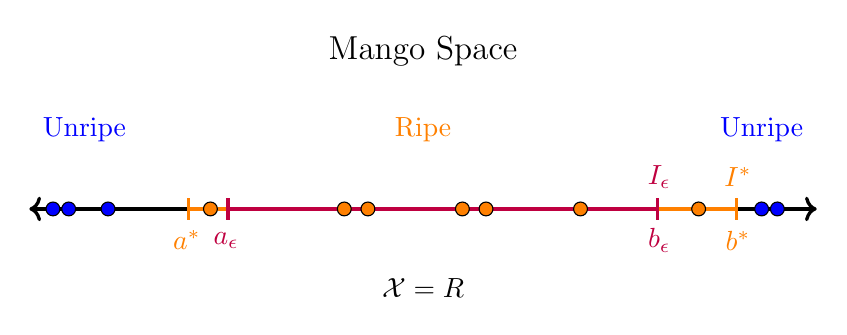
\begin{tikzpicture}
		\draw[<->,very thick] (-5,0) -- (5,0);
		\draw[color = orange, |-|,very thick] (-3,0) -- (4,0);
		\node[color=orange] at (4,.4) {$I^*$};
		\node at (0,2) {\large Mango Space} ;
		\node at (0,-1) {$\mathcal{X} = \mathbb{R}$} ;
		\node [color=blue] at (-4.3,1) {Unripe} ;
		\node [color=blue] at (4.3,1) {Unripe} ;
		\node [color=orange] at (0,1) {Ripe} ;

		\node [color=orange] at (-3,-.4) {$a^*$} ;
		\node [color=orange] at (4,-.4) {$b^*$} ;

		\draw [color=purple, |-|,very thick] (-2.5,0) -- (3,0);
		\node [color=purple] at (3,.4) {$I_\epsilon$} ;
		\node [color=purple] at (-2.5,-.4) {$a_\epsilon$} ;
		\node [color=purple] at (3,-.4) {$b_\epsilon$} ;

%		\draw [color=olive, |-|,very thick] (-3.5,0) -- (2.5,0);
%		\node [color=olive] at (3,.4) {$h_{\mathcal{T}}$} ;



		\node[circle,draw=black, fill=orange, inner sep=0pt,minimum size=5pt] at (2,0) {};
		\node[circle,draw=black, fill=orange, inner sep=0pt,minimum size=5pt] at (-1,0) {};
		\node[circle,draw=black, fill=orange, inner sep=0pt,minimum size=5pt] at (-.7,0) {};
		\node[circle,draw=black, fill=orange, inner sep=0pt,minimum size=5pt] at (.5,0) {};
		\node[circle,draw=black, fill=orange, inner sep=0pt,minimum size=5pt] at (.8,0) {};
		\node[circle,draw=black, fill=orange, inner sep=0pt,minimum size=5pt] at (-2.7,0) {};
		\node[circle,draw=black, fill=orange, inner sep=0pt,minimum size=5pt] at (3.5,0) {};

		\node[circle,draw=black, fill=blue, inner sep=0pt,minimum size=5pt] at (-4.5,0) {};
		\node[circle,draw=black, fill=blue, inner sep=0pt,minimum size=5pt] at (-4,0) {};
		\node[circle,draw=black, fill=blue, inner sep=0pt,minimum size=5pt] at (-4.7,0) {};
		\node[circle,draw=black, fill=blue, inner sep=0pt,minimum size=5pt] at (4.3,0) {};
		\node[circle,draw=black, fill=blue, inner sep=0pt,minimum size=5pt] at (4.5,0) {};
	\end{tikzpicture}
  \end{minipage}
  \vfill
  \begin{minipage}[t][0.5\textheight][t]{\textwidth}
Lets understand this visually.
$$
Err(x_0) = \sigma_\epsilon^2 + [E_\cT[\hat f(x_0)] - f(x_0)]^2 + E_\cT\big[ \hat{f}(x_0) - E_\cT[\hat{f}(x_0)] \big]^2\,.
$$\pause
Consider a data set, 
\end{minipage}
\end{frame}


\begin{frame}[fragile]{Point Variance of Linear Predictor}
Since $x_0^T  (\bfX^T\bfX)^{-1}\bfX^T\epsilon$ is a vector, squaring it is the same as multiply by its transpose. \pause This allow us to write
\begin{align*}
\action<+->{\textbf{Var} &= E_\cT\big[(\,x_0^T  (\bfX^T\bfX)^{-1}\bfX^T\epsilon\,)^2\big] && \text{From before,}}
\\
\action<+->{  &=   E_\cT\big[(\,x_0^T  (\bfX^T\bfX)^{-1}\bfX^T\epsilon\,)(\,x_0^T  (\bfX^T\bfX)^{-1}\bfX^T\epsilon\,)^T\big]  && }
\\
\action<+->{  &=   E_\cT\big[(\,x_0^T  (\bfX^T\bfX)^{-1}\bfX^T\epsilon\,)(\epsilon^T \bfX (\bfX^T\bfX)^{-1} \,x_0)\big] &&  }
\\
\action<+->{  &= (\,x_0^T  (\bfX^T\bfX)^{-1}\bfX^T) E_\cT[\epsilon\epsilon^T] (\bfX (\bfX^T\bfX)^{-1} x_0)  &&\bfX,\,x_0\,\text{const,}}
\\
\action<+->{  &=  (\,x_0^T  (\bfX^T\bfX)^{-1}\bfX^T)\,(\sigma_\epsilon^2 I)\, (\bfX (\bfX^T\bfX)^{-1} x_0)  && \text{Def. of Var,} }
\\
\action<+->{  &=  \sigma^2_\epsilon \, \,x_0^T  (\bfX^T\bfX)^{-1}x_0  && \text{Simplify.} }
\end{align*}
\action<+->{The variance is proportional to the variance in the random variable. But how do we understand the matrix $(\bfX^T\bfX)^{-1}$?}
\end{frame}







\begin{frame}[fragile]{Binary Classification}
  \begin{minipage}[t][0.5\textheight][t]{\textwidth}
	\centering \includegraphics[height=0.5\textheight]{L9BC2.png} 
  \end{minipage}
  \vfill
\begin{minipage}[t][0.5\textheight][t]{\textwidth}
In binary classification, the target space $\mathcal{Y}$ is a categorical variable with two labels. \pause For example, the data above (UW Breast Cancer Dataset) is attempting to classify tumor cells as malignant or nonmalignant based on the cells average area and average concavity. 

\end{minipage}
\end{frame}



















